\documentclass[11pt,a4paper]{article}

% ---------------------------------------------------------------------------
% Counterfactual Goalkeeper Positioning from StatsBomb Event Data
% Math and Machine Learning Praktikum, University of Leipzig
% Compile: pdflatex report && bibtex report && pdflatex report && pdflatex report
% (or use latexmk -pdf report). No local TeX here; Overleaf-ready.
% ---------------------------------------------------------------------------

\usepackage[utf8]{inputenc}
\usepackage[T1]{fontenc}
\usepackage{lmodern}
\usepackage[margin=2.5cm]{geometry}
\usepackage{amsmath,amssymb}
\usepackage{graphicx}
\usepackage{booktabs}
\usepackage{caption}
\usepackage{subcaption}
\usepackage{siunitx}
\usepackage{xcolor}
\usepackage[numbers,round]{natbib}
\usepackage[colorlinks=true,linkcolor=blue,citecolor=blue,urlcolor=blue]{hyperref}
\hfuzz=1pt  % don't warn about sub-1pt overfulls (unbreakable file paths); cosmetic only

\graphicspath{{figures/}}
\captionsetup{font=small}

\newcommand{\gopt}{g^{*}}
\newcommand{\V}{V}
\newcommand{\argmin}{\operatorname*{arg\,min}}

\title{\textbf{Counterfactual Goalkeeper Positioning\\ from Football Event Data}}
\author{Lauren Pommer\\[2pt]
  \small in collaboration with Hannes\\
  \small Math and Machine Learning Praktikum, University of Leipzig}
\date{\today}

\begin{document}
\maketitle

\begin{abstract}
\noindent
We build a counterfactual model of goalkeeper positioning,
$\V(x,g)=P(\text{goal}\mid x,g)$, that estimates goal probability from the
non-goalkeeper context of a shot $x$ and a hypothetical goalkeeper position $g$.
Holding $x$ fixed and sweeping $g$ over a pitch grid turns a descriptive
expected-goals model into a \emph{prescriptive} one: the recommended position is
$\gopt=\argmin_g \V(x,g)$, and a keeper's \emph{regret} is
$\V(x,g_{\text{actual}})-\V(x,\gopt)$. Training a convolutional network on
\num{30000} men's open-play shots from the StatsBomb open data, a purely spatial
model (\texttt{v1}) is already competitive with the built-in StatsBomb xG on
ranking and calibration (AUC \num{0.803}, ECE \num{0.010}). However, its
counterfactual recommendations are pathological: lacking any structural
knowledge of the goal frame, $\gopt$ pins to grid boundaries and, for wide
shots, recommends the \emph{far} post --- the opposite of coaching intuition.
We show this is a causal failure of an observational model and fix it with
inductive biases: five static goal-geometry channels and a spatial-preserving
pool (\texttt{v2}) yield clean, grid-independent recommendations
(anti-coaching optima $0.2\%\pm0.45\%$ over five seeds) that remain valid under
domain shift to women's and other men's competitions. Adding a parallel
scalar-feature head (\texttt{v3}) closes the small residual gap to StatsBomb xG
(AUC $0.819\pm0.001$) but degrades and destabilises the counterfactual policy;
we trace this to \emph{training interference} rather than the inference-time
features, and argue that a single model cannot be both the best predictor and
the best positioning recommender under this architecture. We report the tension
itself as a contribution.
\end{abstract}

% ===========================================================================
\section{Introduction}
% ===========================================================================

Expected-goals (xG) models estimate how dangerous a shot was. They are
\emph{descriptive}: given a shot, they return a probability of a goal. A natural
and more useful question for goalkeeper analysis is \emph{prescriptive}: given
everything else about a shot, where \emph{should} the goalkeeper have stood to
minimise the chance of conceding? This report develops a model that answers the
prescriptive question by treating the goalkeeper's position as an intervenable
variable.

Let $Y\in\{0,1\}$ be the shot outcome ($1$ = goal), let $g\in\mathbb{R}^2$ be the
goalkeeper's position, and let $x$ denote everything else in the recorded scene
at the moment of the shot (shooter and ball, attacking teammates, outfield
defenders). We learn the conditional probability
\begin{equation}
  \V(x,g) = P(Y=1\mid x,g),
\end{equation}
and, at inference, fix the observed context $x$ and minimise over hypothetical
goalkeeper positions,
\begin{equation}
  \gopt(x) = \argmin_{g\in\mathcal{G}} \V(x,g),
  \label{eq:gstar}
\end{equation}
producing a danger heatmap over the pitch and a single recommended position.

\paragraph{Contributions.}
\begin{enumerate}\itemsep2pt
  \item A convolutional model over a rasterised pitch that estimates $\V(x,g)$
        and is competitive with StatsBomb's xG using \emph{only} player
        positions --- no distance, angle, body part or pressure features
        (Section~\ref{sec:results-pred}).
  \item A diagnosis of why a purely spatial model produces
        counterfactually invalid recommendations: it learns the observational
        correlation ``keeper in the goal mouth $\Rightarrow$ goal conceded'' and
        so $\gopt$ drifts off the goal line
        (Section~\ref{sec:results-v1cf}).
  \item An inductive-bias fix (goal-geometry channels + a spatial pool) that
        yields clean, grid-independent, and \emph{domain-invariant}
        recommendations (Sections~\ref{sec:results-v2}--\ref{sec:results-transfer}).
  \item Evidence of a \emph{predictive-versus-counterfactual tension}: a
        parallel scalar head improves prediction but degrades the positioning
        policy, and the cause is training interference, not the added features
        (Section~\ref{sec:results-tension}).
\end{enumerate}

% ===========================================================================
\section{Background and Related Work}
% ===========================================================================

\paragraph{Expected goals.}
StatsBomb's event data ships a built-in xG value for every shot, which we use as
an external benchmark. \citet{anzer2021goal} build a goal-probability model on
synchronised Bundesliga tracking data, reporting a ranked probability score of
\num{0.197}; their inputs include full optical tracking of all players. Our
setting is more constrained: the StatsBomb shot-event freeze frames annotate only
players near the shot (Section~\ref{sec:data}), so our context $x$ is
noisier and less complete than tracking data.

\paragraph{From prediction to prescription.}
A calibrated xG model is descriptive. The counterfactual sweep of
Eq.~\eqref{eq:gstar} upgrades it to a prescriptive statement about goalkeeper
positioning. In the language of \citet{pearl2009causality}, evaluating
$\V(x,g)$ over hypothetical $g$ is an intervention $do(G=g)$ on a single
variable; it is only a valid counterfactual if the model has learned the true
conditional probability \emph{and} extrapolates sensibly to $(x,g)$ pairs that
are unsupported in the training distribution. A central finding of this report
is that the second condition fails for a naive spatial model and must be
engineered in.

\paragraph{Inductive biases.}
Our fix rests on two classical ideas. Convolutions encode locality and
translation equivariance, which match the physics of shot danger (local
shooter--keeper geometry, evaluated the same way anywhere on the pitch). But
translation equivariance also \emph{removes} absolute position, which the goal
frame depends on; we restore it with explicit coordinate channels in the spirit
of CoordConv \citep{liu2018coordconv} together with an explicit goal-frame
channel.

% ===========================================================================
\section{Data}
\label{sec:data}
% ===========================================================================

We use the StatsBomb open data \citep{statsbomb_opendata}, accessed through the
\texttt{mplsoccer} parser. Each shot carries an event record (location, outcome,
xG, body part, pressure) and a \emph{freeze frame}: the annotated positions of
players at the instant of the shot.

\paragraph{Freeze-frame caveat.}
These are StatsBomb's older shot-event freeze frames, not StatsBomb~360. They are
manually annotated and scoped to players in the vicinity of the shot, with no
\texttt{visible\_area} polygon. A player absent from a freeze frame therefore
means ``not annotated near the shot,'' not ``confirmed absent from the pitch.''
The median frame contains \num{13} players (range \numrange{1}{21}), so context
completeness varies across shots --- more so than in the tracking-data setting of
\citet{anzer2021goal}. Crucially for this project, the goalkeeper is present in
\SI{99.9}{\percent} of open-play frames, so the position signal we optimise over
is reliable.

\paragraph{Scope and sample.}
We restrict to open-play shots (excluding set pieces, penalties and direct free
kicks). Of \num{87111} shots, \num{81551} (\SI{93.6}{\percent}) are open play,
and \num{81453} (\SI{99.9}{\percent}) have an identifiable opponent goalkeeper;
this is our modelling sample. The open-play conversion rate is
\SI{10.3}{\percent}, i.e.\ a strongly imbalanced rare-event problem.

\paragraph{Splits.}
To measure generalisation under domain shift, we split by competition rather than
at random. Men's 2015/16 top-five European leagues form the in-domain
train/validation/test sets (\num{30000}/\num{6400}/\num{6500} shots); women's
competitions (\num{12600}) and all other men's competitions (\num{25800}) are
held out entirely as transfer sets. Goal rates are consistent across splits
(\SIrange{9.7}{10.3}{\percent}). Figure~\ref{fig:eda} shows where shots occur and
confirms the class imbalance.

\begin{figure}[t]
  \centering
  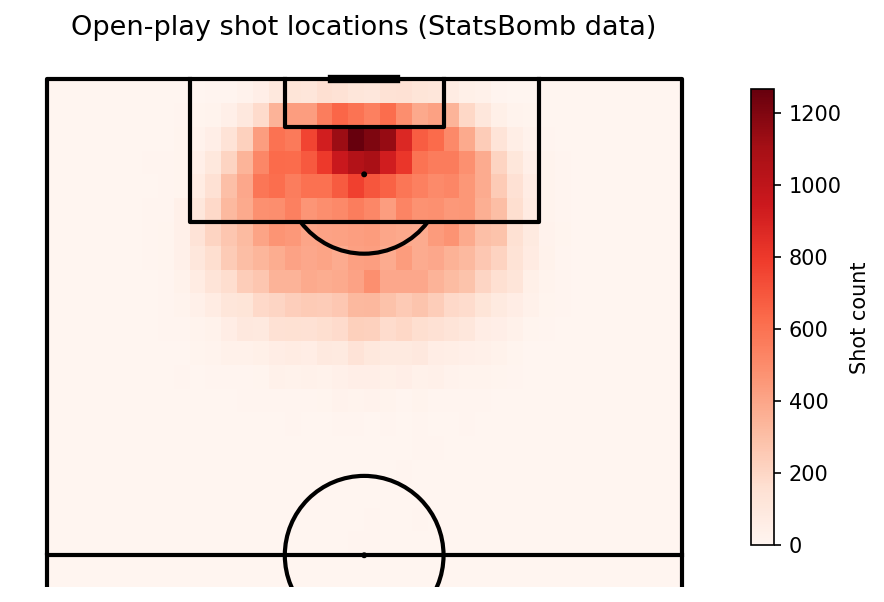
\includegraphics[width=0.62\linewidth]{eda_shot_heatmap.png}
  \caption{Shot locations in the open-play sample (attacking towards the right
    goal). Shots concentrate in and around the penalty area, motivating the
    cropped pitch region used for rasterisation.}
  \label{fig:eda}
\end{figure}

% ===========================================================================
\section{Method}
\label{sec:method}
% ===========================================================================

\subsection{Learning problem}
We estimate $\V(x,g)=P(Y=1\mid x,g)$ by binary classification. A network
$f_\theta$ outputs a logit that is passed through a sigmoid $\sigma$ and trained
with binary cross-entropy,
\begin{equation}
  \mathcal{L}(\theta) = -\frac{1}{N}\sum_{i=1}^{N}
    \Big[ y_i \log \sigma(f_\theta(z_i)) + (1-y_i)\log\big(1-\sigma(f_\theta(z_i))\big)\Big],
  \label{eq:bce}
\end{equation}
where $z_i$ is the rasterised representation of shot $i$
(Section~\ref{sec:raster}). BCE is the negative log-likelihood of a Bernoulli
model; under a rich enough function class its population minimiser is the true
conditional probability $P(Y=1\mid z)$. This is what licenses reading
$\sigma(f_\theta(z))$ as a probability, and why we treat \emph{calibration}
(Brier score \citep{brier1950verification}, expected calibration error
\citep{guo2017calibration}) as a first-class metric alongside ranking (AUC): the
sweep in Eq.~\eqref{eq:gstar} takes an $\argmin$ over absolute probabilities, so
mis-calibrated outputs would corrupt $\gopt$.

\subsection{Input representation}
\label{sec:raster}
Each shot is rasterised onto an $80\times 60$ grid covering the attacking third
($x\in[60,120]$, \SI{1}{m} per cell). Every relevant player is rendered as a 2D
isotropic Gaussian
\begin{equation}
  K_\sigma(u;p) = \exp\!\Big(-\tfrac{\lVert u-p\rVert^2}{2\sigma^2}\Big),
  \qquad \sigma\approx\SI{1.5}{m},
\end{equation}
with $\sigma$ absorbing annotation noise. The five \emph{player channels} are:
shooter, ball, attacking teammates, outfield defenders, and goalkeeper. The two
crowd channels (teammates, defenders) are max-pooled rather than summed, keeping
their amplitude in $[0,1]$ regardless of how many players are annotated.
Figure~\ref{fig:raster} shows an example.

\begin{figure}[t]
  \centering
  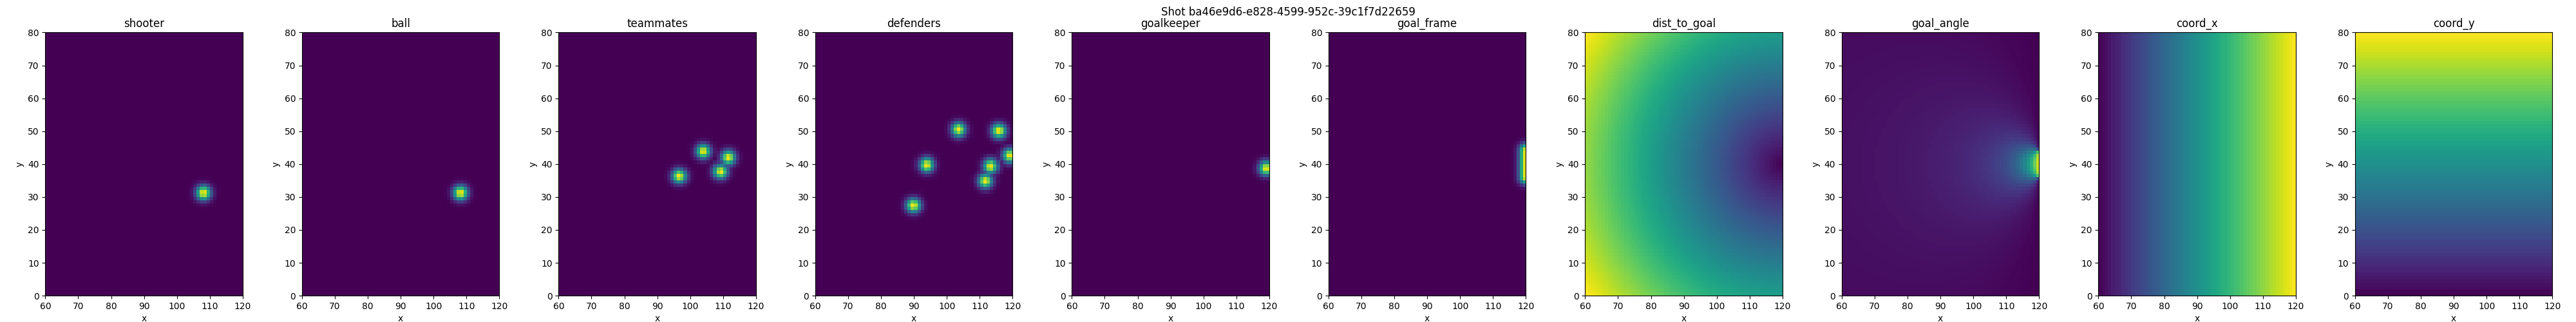
\includegraphics[width=0.95\linewidth]{rasterize_example.png}
  \caption{Rasterised representation of one shot. The model sees only these
    channels: player positions as Gaussian blobs (plus, in \texttt{v2}, static
    goal-geometry channels described in Section~\ref{sec:v2}). The goalkeeper
    channel is the variable swept at inference.}
  \label{fig:raster}
\end{figure}

\subsection{Architecture}
The \texttt{DangerCNN} backbone is three \texttt{Conv--BatchNorm--ReLU} blocks
\citep{ioffe2015batchnorm} with intervening max-pools, followed by an adaptive
average pool, two fully connected layers and a sigmoid. Convolutional weights use
He initialisation \citep{he2015delving}; we train with Adam
\citep{kingma2015adam}, weight decay \num{1e-5}, dropout \num{0.3}, and early
stopping on validation loss. The parameter budget is kept between roughly
\num{100}k and \num{200}k to limit overfitting on \num{30000} shots. We
study three variants, summarised in Table~\ref{tab:variants}.

\begin{table}[t]
  \centering
  \small
  \begin{tabular}{@{}lp{9.6cm}r@{}}
    \toprule
    Variant & Inputs and head & Params \\
    \midrule
    \texttt{v1} & 5 player channels; global average pool & \num{102}k \\
    \texttt{v2} & + 5 static goal-geometry channels; $(4,3)$ spatial pool & \num{194}k \\
    \texttt{v3} & \texttt{v2} + parallel scalar-feature head (9 features) & \num{196}k \\
    \bottomrule
  \end{tabular}
  \caption{Model variants. \texttt{v2} adds structural priors to \texttt{v1};
    \texttt{v3} adds a hand-engineered scalar head on top of \texttt{v2}. A
    fourth variant \texttt{v3b} restricts the scalar head to the six
    goalkeeper-independent features.}
  \label{tab:variants}
\end{table}

\subsection{Goal-geometry channels and the spatial pool}
\label{sec:v2}
Variant \texttt{v2} appends five \emph{static} channels (identical for every
shot) that make the goal frame explicit: a Gaussian ridge on the goal-line
segment between the posts (\texttt{goal\_frame}); normalised distance to goal;
the angle subtended by the two posts as seen from each cell (view angle); and two
normalised coordinate channels $(x,y)$ in the CoordConv sense
\citep{liu2018coordconv}. In addition, \texttt{v1}'s global average pool --- which
discards absolute position by construction --- is replaced by a small $(4,3)$
adaptive pool, so a coarse spatial layout survives into the classifier. Both
changes give the model the ability to reason about \emph{where} the goal is,
which Section~\ref{sec:results-v1cf} shows is exactly what \texttt{v1} lacks.

\subsection{Scalar-feature head}
Variant \texttt{v3} adds a parallel multilayer perceptron over nine
hand-engineered scalars (distance, shot angle, goalkeeper angular coverage of the
goal, keeper perpendicular offset and depth, three body-part indicators, and an
under-pressure flag), concatenated with the convolutional embedding before the
output layer. Three of the nine features depend on the goalkeeper; the
\emph{context} subset \texttt{v3b} keeps only the six that do not.

\subsection{Counterfactual sweep and regret}
\label{sec:sweep}
To evaluate Eq.~\eqref{eq:gstar} we fix all non-goalkeeper channels, then for
each candidate $g$ in a grid $\mathcal{G}$ we overwrite the goalkeeper channel
with a Gaussian centred at $g$ and forward the network, yielding a danger
heatmap. We use a physically constrained grid --- $x\in[108,120]$ (penalty spot
to goal line), $y\in[34,46]$ (posts at $y\in\{36,44\}$ plus a \SI{2}{m} diving
margin), \SI{0.5}{m} step --- and contrast it with the wider grid
$x\in[110,120]$, $y\in[30,50]$ used to expose the \texttt{v1} pathology. The cost
is a few hundred forward passes per shot ($\sim$\num{5}~MFLOPs each).

For a shot with observed goalkeeper position $g_{\text{actual}}$, the
\emph{regret} is
\begin{equation}
  R(x) = \V(x,g_{\text{actual}}) - \V(x,\gopt)
       = \V(x,g_{\text{actual}}) - \min_{g\in\mathcal{G}}\V(x,g) \; \ge 0 .
  \label{eq:regret}
\end{equation}
Regret factors out intrinsic shot difficulty: a breakaway may have high
$\V(x,g_{\text{actual}})$ yet near-zero regret (no position helps), whereas a
shot from a tight angle may have moderate $\V$ but large regret (a better
position would have removed most of the danger).

\paragraph{Counterfactual-quality metrics.}
Because regret is only trustworthy when $\gopt$ is physical, we score the
\emph{policy} $\gopt$ directly over a fixed seeded sample of \num{200} shots. We
report the fraction of optima that (i) pin to the $y$-edge of the grid (the
\texttt{v1} failure mode), and (ii) land on the \emph{far} side of the shooter
--- behind the post opposite the ball, the anti-coaching signal --- together with
a near/centre/far breakdown. A good positioning recommender should have both
rates near zero.

% ===========================================================================
\section{Results}
% ===========================================================================

\subsection{Predictive accuracy}
\label{sec:results-pred}
Table~\ref{tab:pred} reports test-set metrics. The purely spatial \texttt{v1} is
already competitive with StatsBomb's xG on ranking and is very well calibrated
(ECE \num{0.010}), with a Pearson correlation of \num{0.74} to StatsBomb xG ---
agreement in direction, but independent in absolute terms. Adding goal-geometry
channels (\texttt{v2}) improves AUC to $0.814\pm0.003$ while preserving
calibration. The scalar head (\texttt{v3}) reaches $0.819\pm0.001$, matching
StatsBomb xG (\num{0.821}). We deliberately do \emph{not} rebalance the classes:
the rare-event base rate is what makes the outputs calibrated probabilities, and
BCE already targets the correct conditional (Section~\ref{sec:method}); a check
confirmed the validation plateau (Figure~\ref{fig:curves}) is ordinary
overfitting, not imbalance starvation.

\begin{table}[t]
  \centering
  \small
  \begin{tabular}{@{}lcccl@{}}
    \toprule
    Model & AUC & Brier & ECE & Notes \\
    \midrule
    StatsBomb xG           & 0.821 & --- & --- & external benchmark \\
    \texttt{v1}            & 0.803 & 0.075 & 0.010 & spatial only, global pool \\
    \textbf{\texttt{v2}}   & $\mathbf{0.814\pm0.003}$ & $0.0716$ & $0.0077$ & 5-seed; \textbf{recommended} \\
    \texttt{v3} (all)      & $0.819\pm0.001$ & $0.0704$ & $0.0097$ & 5-seed; $\approx$ StatsBomb xG \\
    \texttt{v3b} (context) & 0.815 & 0.0708 & 0.0065 & single seed; best ECE \\
    \bottomrule
  \end{tabular}
  \caption{Predictive metrics on the in-domain test split. Multi-seed entries are
    mean over five seeds; standard deviations for Brier/ECE are below the last
    reported digit unless shown. Higher AUC is better; lower Brier/ECE is better.}
  \label{tab:pred}
\end{table}

\begin{figure}[t]
  \centering
  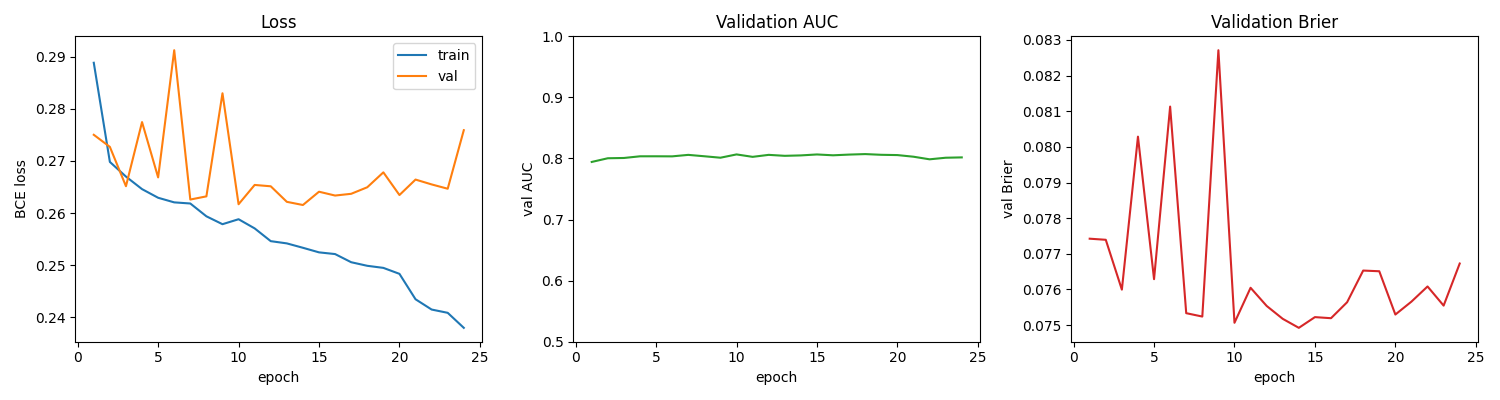
\includegraphics[width=0.8\linewidth]{v2_training_curves.png}
  \caption{Training dynamics for \texttt{v2}. Validation loss plateaus after a few
    epochs while training loss keeps falling --- the overfitting signature that
    motivates the constrained parameter budget and early stopping, rather than a
    symptom of the class imbalance.}
  \label{fig:curves}
\end{figure}

\subsection{The counterfactual pathology of a purely spatial model}
\label{sec:results-v1cf}
Running the sweep on \texttt{v1} exposes a structural failure. Under the wide
grid, $7/8$ example optima pin to the $y$-boundary, \SIrange{2}{4}{m}
\emph{behind} the goal posts; under the constrained grid, $2/8$ still pin at the
edge, and widening those shots further lets $\gopt$ walk outward without bound
(the finite difference $\V(33)-\V(35)<0$: the minimum is a truncation, not an
interior solution). For a wide shot the model recommends the keeper stand behind
the \emph{far} post, opposite the ball --- the reverse of what a coach would say.

The cause is not a bug but a missing inductive bias. \texttt{v1} has no
representation of the goal frame; it only learns the observational regularity
that goalkeepers who conceded were standing inside the goal mouth. Moving the
synthetic keeper \emph{out} of that region therefore lowers $\V$ regardless of
football reality. This is a textbook causal failure of an observational model:
$\V(x,g)$ is a good conditional probability on the training support, but the
$\argmin$ in Eq.~\eqref{eq:gstar} pushes off that support, where the model's
extrapolation has the wrong sign.

\subsection{Goal-geometry channels resolve it}
\label{sec:results-v2}
With the goal frame made explicit and absolute position preserved by the spatial
pool, \texttt{v2}'s recommendations become sensible. Over the fixed \num{200}-shot
sample and five seeds, optima that pin to the edge occur $0.7\%\pm0.45\%$ of the
time and anti-coaching (far-side) optima occur $0.2\%\pm0.45\%$ --- effectively
never, and reproducibly so. Wide shots now send $\gopt$ toward the \emph{near}
post and slightly off the line to cut the angle. Figure~\ref{fig:cf} (left)
illustrates a representative case.

\subsection{Predictive-versus-counterfactual tension}
\label{sec:results-tension}
The scalar head buys predictive accuracy at the cost of the positioning policy.
Table~\ref{tab:cf} and Figure~\ref{fig:cf} show the trade-off: \texttt{v3}'s
far-side rate rises to $16.3\%\pm7.3\%$ and its edge-pinning to $9.9\%\pm15.5\%$
(one seed pins \SI{37.5}{\percent} of optima), whereas \texttt{v2} stays near
zero. Two observations sharpen this into a finding.

First, the effect is a \emph{training} phenomenon, not an inference one. The
\texttt{v3b} context features are goalkeeper-independent: they add the same
constant to every grid cell and therefore \emph{cannot} change the $\argmin$ in
Eq.~\eqref{eq:gstar}. Yet \texttt{v3b}'s $\gopt$ still degrades relative to
\texttt{v2}. The only thing that differs is the convolutional trunk's learned
weights: giving the loss an auxiliary head to explain variance lets the conv
layers offload work onto the scalar MLP, so the spatial branch becomes a worse
\emph{function of keeper position}.

Second, the predictive gain is small. With \texttt{v2} and \texttt{v3} both run
over five matched seeds, a paired comparison gives a mean $\Delta\text{AUC}$ of
$+0.0050$ in \texttt{v3}'s favour ($t=2.80$, $p\approx0.049$), driven largely by
a single seed. So \texttt{v3} matches StatsBomb xG, but does \emph{not} decisively
beat \texttt{v2} on prediction, while clearly losing on counterfactual quality.
We therefore recommend \texttt{v2} as the positioning model and cite \texttt{v3}
only as the xG-parity benchmark, and we report the trade-off itself as a result
about auxiliary-head training interference.

\begin{table}[t]
  \centering
  \small
  \begin{tabular}{@{}lccl@{}}
    \toprule
    Model & far-side / anti-coaching & edge-pinned & post-side (centre/near/far) \\
    \midrule
    \textbf{\texttt{v2}}   & $\mathbf{0.2\%\pm0.45\%}$ & $0.7\%\pm0.45\%$ & $\sim$183/17/0 \\
    \texttt{v3} (all)      & $16.3\%\pm7.3\%$ & $9.9\%\pm15.5\%$ & 67/94/39 \\
    \texttt{v3b} (context) & $14\%$ & $1.5\%$ & 79/93/28 \\
    \bottomrule
  \end{tabular}
  \caption{Counterfactual-quality metrics over a fixed \num{200}-shot sample.
    Multi-seed entries are mean$\pm$std over five seeds. Lower is better;
    \texttt{v2} is both the lowest and the most stable.}
  \label{tab:cf}
\end{table}

\begin{figure}[t]
  \centering
  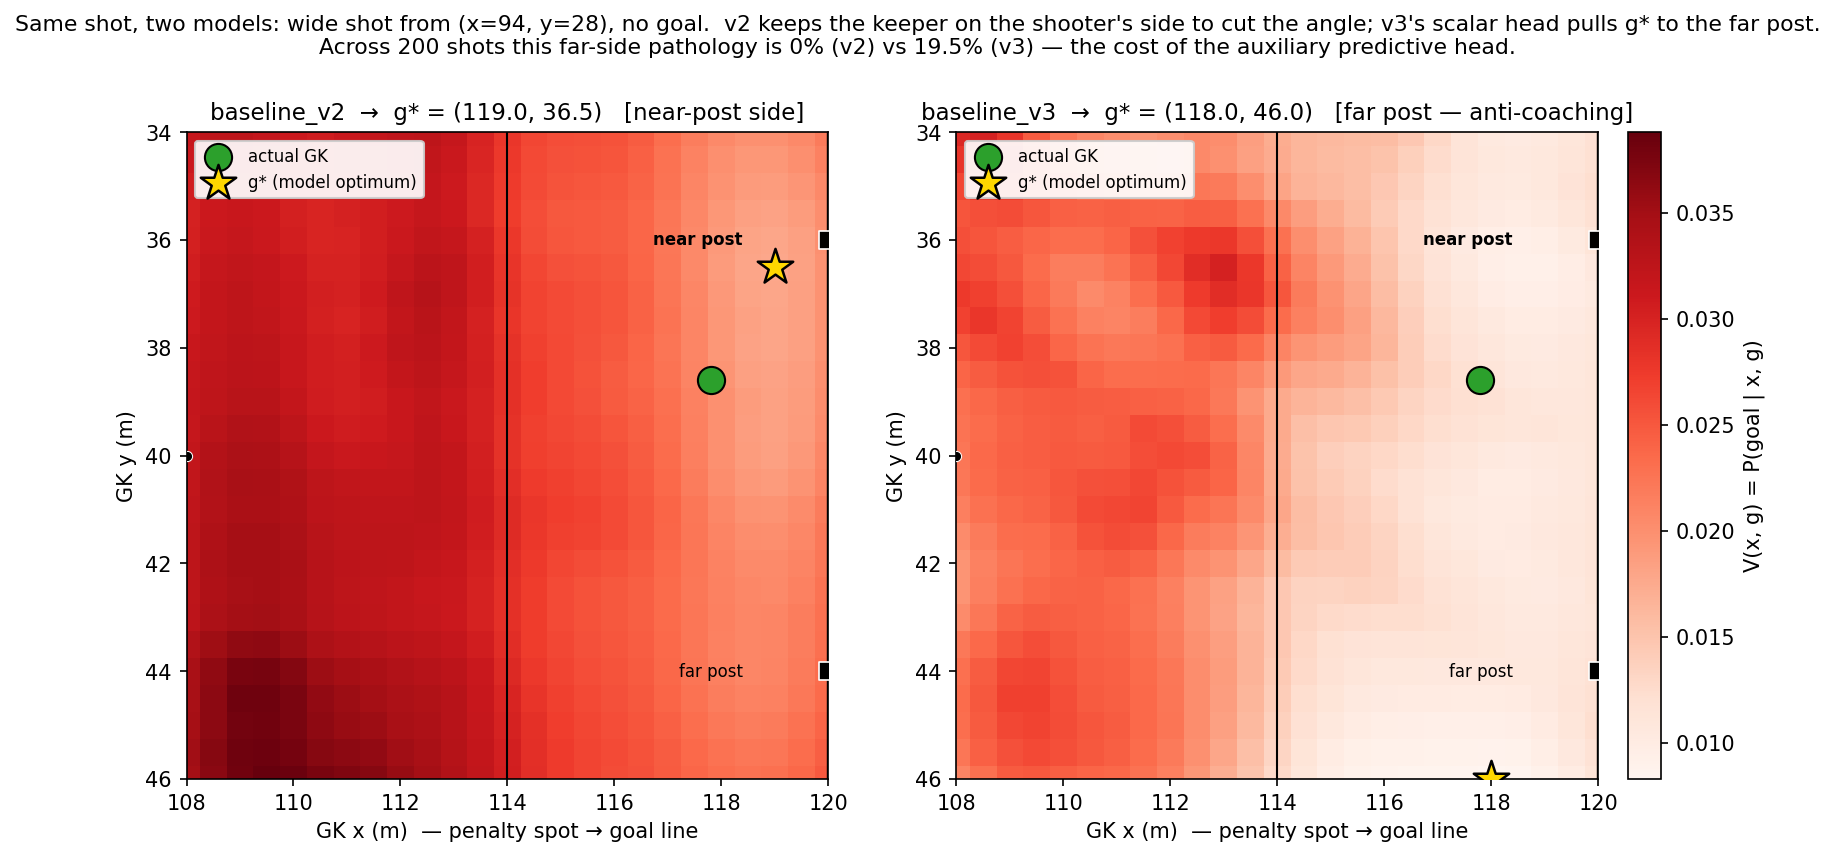
\includegraphics[width=0.99\linewidth]{cf_v2_vs_v3_1e582bc0.png}
  \caption{The same wide shot swept under \texttt{v2} (left) and \texttt{v3}
    (right) on a shared colour scale. \texttt{v2} keeps $\gopt$ on the shooter's
    (near-post) side to cut the angle; \texttt{v3}'s scalar head pulls $\gopt$ to
    the far post. Across \num{200} shots this far-side pathology is
    \SI{0.2}{\percent} (\texttt{v2}) versus \SI{16.3}{\percent} (\texttt{v3}).}
  \label{fig:cf}
\end{figure}

\begin{figure}[t]
  \centering
  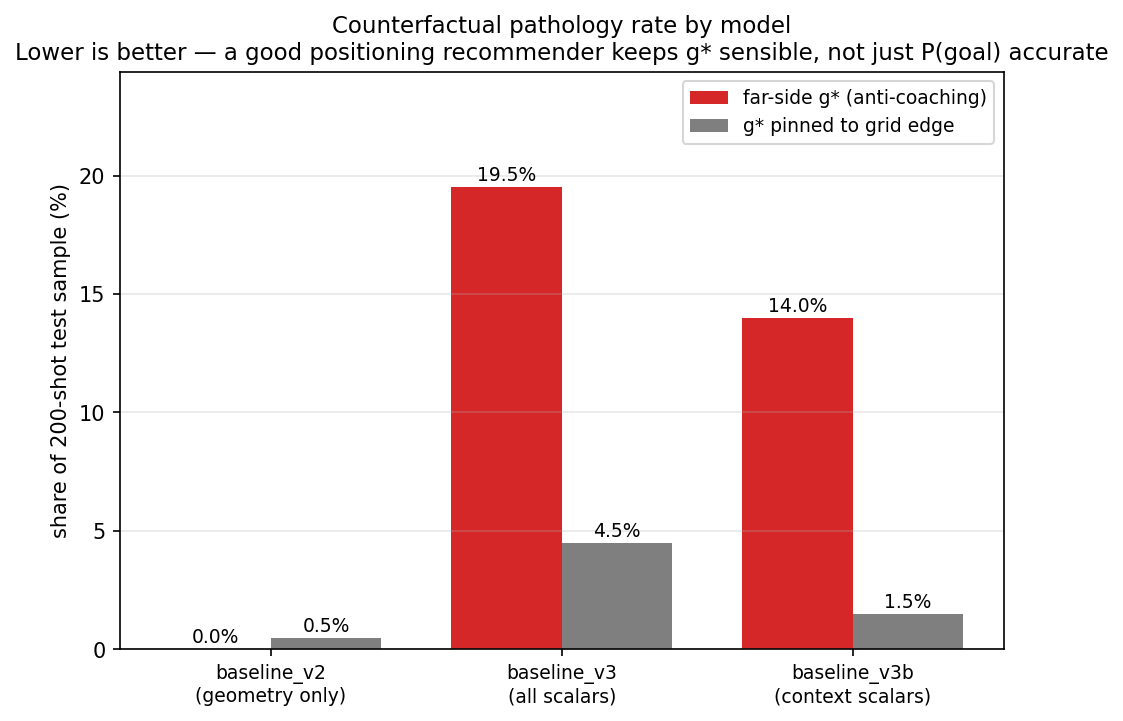
\includegraphics[width=0.62\linewidth]{far_side_by_model.png}
  \caption{Counterfactual pathology rate by model over the \num{200}-shot sample.
    A good positioning recommender keeps $\gopt$ sensible, not merely $P(\text{goal})$
    accurate.}
  \label{fig:barchart}
\end{figure}

\subsection{Validation: multi-seed stability and transfer}
\label{sec:results-transfer}
The clean-counterfactual property of \texttt{v2} is reproducible across five
seeds (Table~\ref{tab:cf}) rather than a lucky run. It also survives domain
shift. Evaluated out-of-domain, \texttt{v2}'s predictive AUC drops as expected
(in-domain \num{0.809}, women \num{0.781}, other men \num{0.797}) but its gap to
StatsBomb xG stays stable ($\sim$\numrange{0.012}{0.014} AUC) and calibration
stays within \num{1.7}~pp. Critically, the counterfactual policy stays clean:
far-side optima remain near zero out-of-domain (women \SI{0}{\percent}, other men
\SI{1}{\percent}). The goal-frame geometry that drives $\gopt$ is
domain-invariant even where raw $P(\text{goal})$ accuracy is not.

\subsection{Augmentation: position jitter}
Following a suggestion to augment with perturbed positions, we trained
\texttt{v2} with train-only Gaussian jitter ($\sigma=\SI{0.75}{m}$) on every
player, resampled each epoch. The result is neutral: predictive and
counterfactual metrics are unchanged, and, measured directly, the roughness of
the danger landscape (mean total variation of the grid) is identical
(\num{0.0053} vs \num{0.0053}). The geometry channels already yield a smooth
$\V(x,g)$, so there was no brittleness for jitter to remove --- a useful negative
control and a robustness check that \texttt{v2}'s $\gopt$ survives perturbing
every training position.

\subsection{What the representation encodes}
To see what \texttt{v2} learned, we take the \num{64}-dimensional embedding just
before the output layer, run it over the test split, and project to two
dimensions with PCA (Figure~\ref{fig:latent}). The first principal component
explains \SI{48.7}{\percent} of the variance and is essentially a
\emph{danger axis}: it correlates $-0.85$ with predicted $P(\text{goal})$,
$-0.72$ with StatsBomb xG, and $+0.68$ with shooter-to-goal distance, and goals
concentrate in its low tail. The model organises its representation around danger
and geometry rather than raw player density --- consistent with the geometry
channels doing the intended work.

\begin{figure}[t]
  \centering
  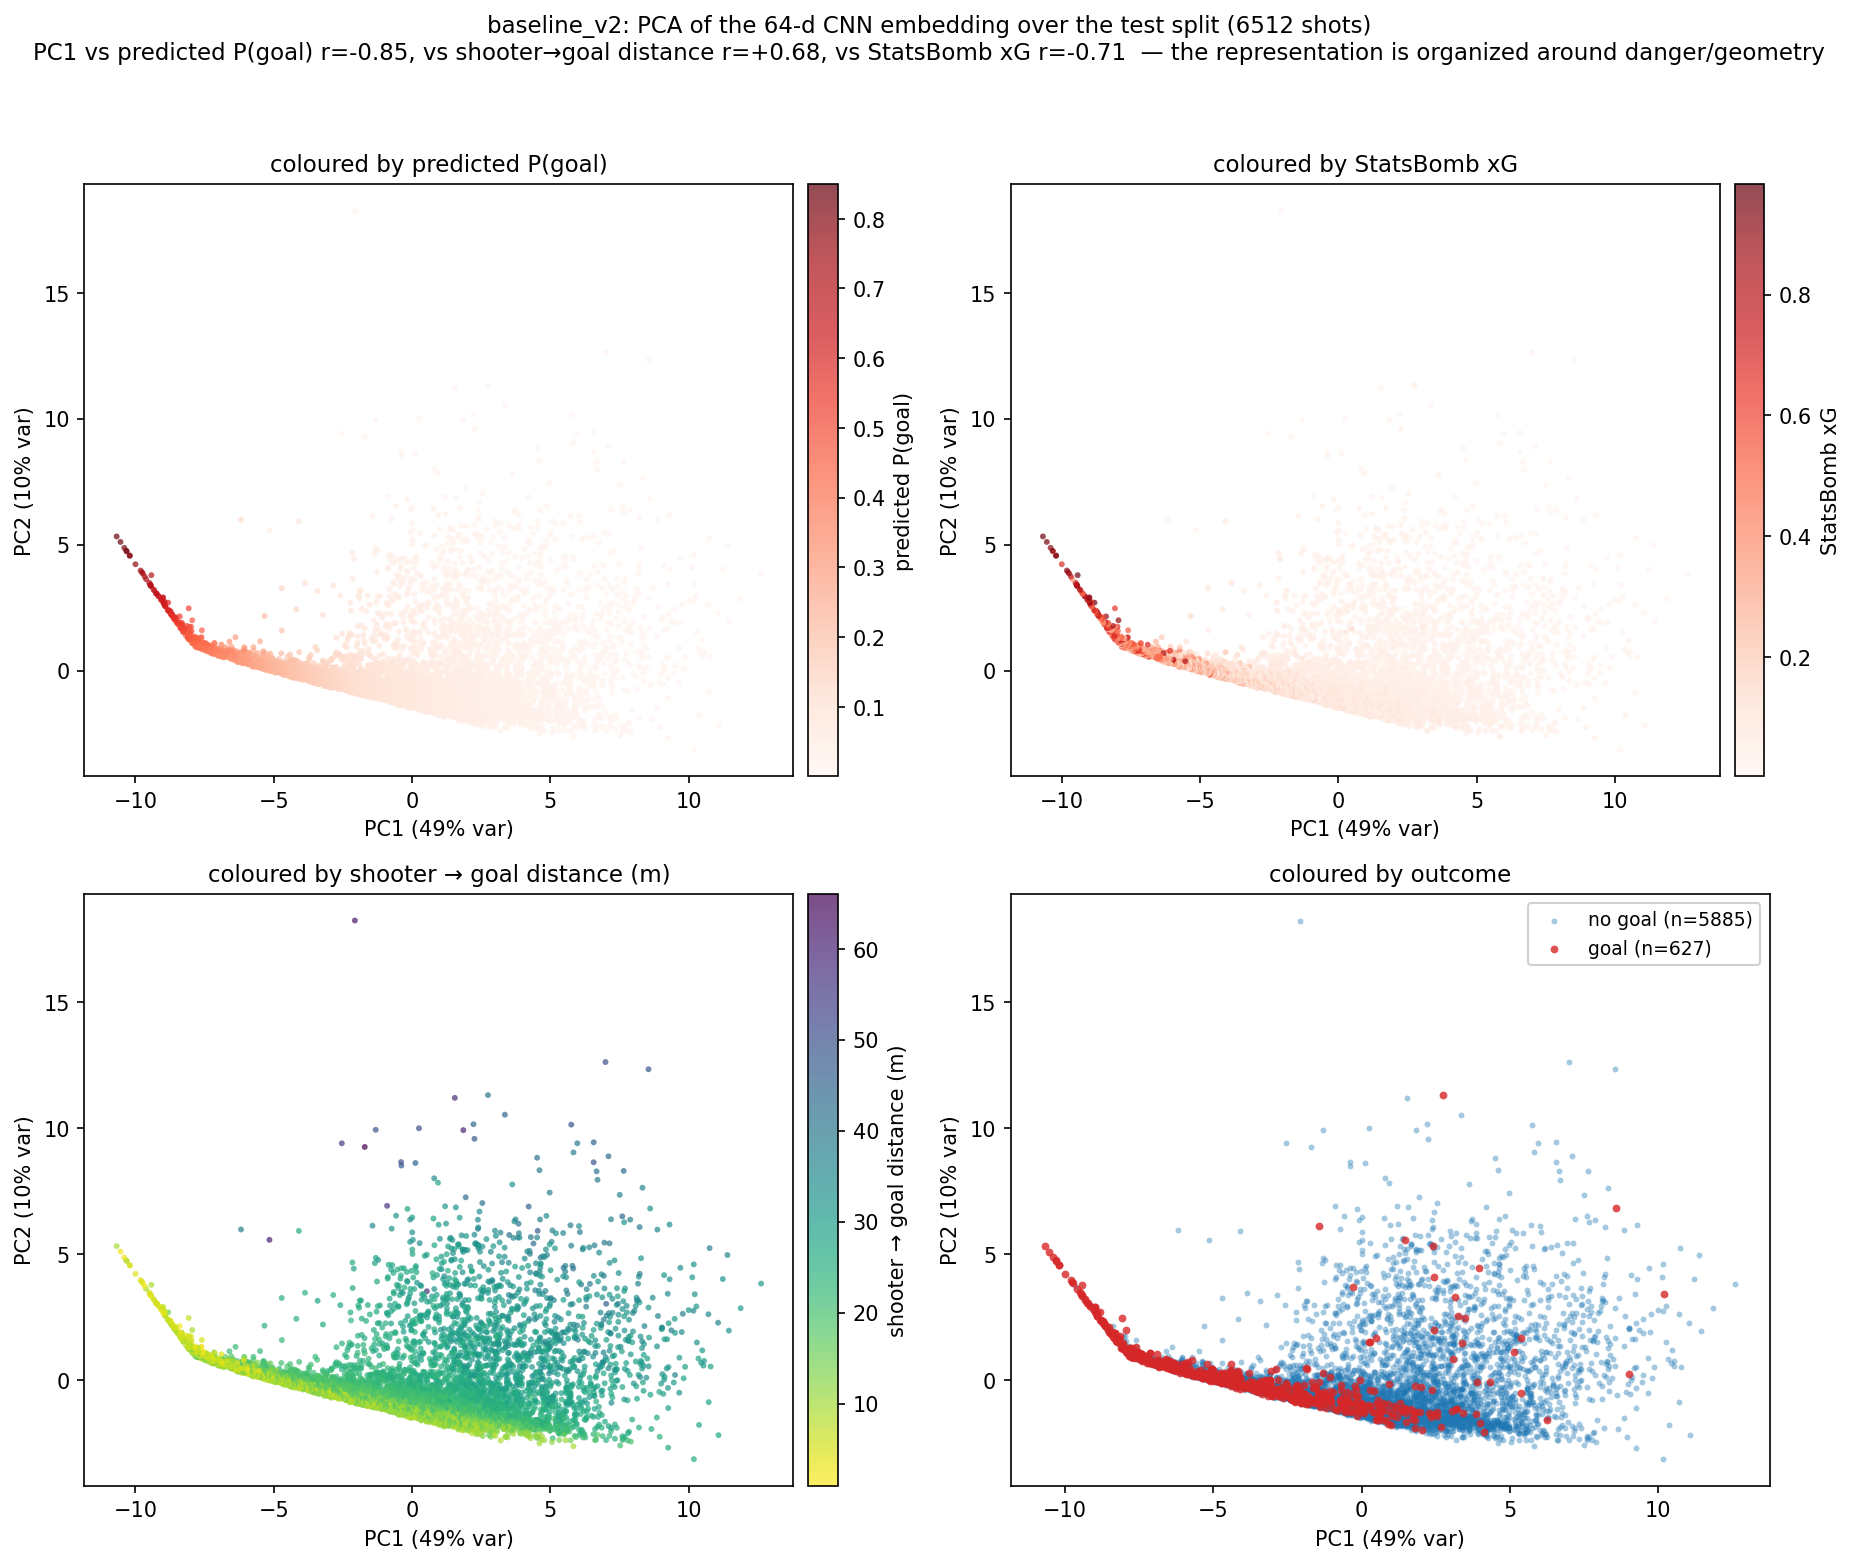
\includegraphics[width=0.85\linewidth]{latent_embedding_v2.png}
  \caption{PCA of \texttt{v2}'s \num{64}-d embedding over the test split, coloured
    by predicted $P(\text{goal})$, StatsBomb xG, shooter--goal distance, and
    outcome. PC1 is a smooth danger axis.}
  \label{fig:latent}
\end{figure}

% ===========================================================================
\section{Discussion}
% ===========================================================================

\paragraph{A descriptive model is not automatically prescriptive.}
The \texttt{v1}$\rightarrow$\texttt{v2} story is the methodological core of this
project. A well-calibrated conditional probability can still yield nonsensical
recommendations, because the recommendation is an $\argmin$ over inputs the model
was never trained on. Making the sweep valid required a structural prior (the
goal frame), not more data or a better fit.

\paragraph{One model cannot be both.}
The \texttt{v2}/\texttt{v3}/\texttt{v3b} comparison shows that pushing predictive
accuracy via an auxiliary head interferes with the spatial branch that carries
the positioning policy --- even when the added features provably cannot change
$\gopt$. The pragmatic resolution is to use two models for two purposes:
\texttt{v2} to recommend $\gopt$, \texttt{v3} (or StatsBomb xG) to report an
absolute danger number.

\paragraph{Limitations.}
The freeze frames are partial and manually annotated, so context $x$ is
incomplete for some shots (Section~\ref{sec:data}). Regret magnitudes inherit
whatever residual bias remains in $\gopt$; we treat comparative regret (which
shots have positional slack) as more reliable than absolute regret. Finally, the
constrained sweep grid encodes a modelling choice about the physical range of
keeper positions; \texttt{v2} no longer pins to its edges, which makes the choice
far less load-bearing than it was for \texttt{v1}, but it remains a choice.

% ===========================================================================
\section{Conclusion and Future Work}
% ===========================================================================

We built a counterfactual goalkeeper-positioning model and showed that the step
from a descriptive xG-style network to a valid positioning recommender is an
inductive-bias problem, not a capacity or data problem. Goal-geometry channels
and a spatial pool (\texttt{v2}) produce clean, reproducible, domain-invariant
recommendations, while a predictive scalar head (\texttt{v3}) closes the last gap
to StatsBomb xG at the cost of the positioning policy --- a training-interference
trade-off we report as a finding.

The most promising next step is a single spatial channel encoding defender
occlusion of the shot cone. Because it enters through the convolutional pathway
rather than a parallel head, it directly tests whether it is the extra
information or the parallel head that harms $\gopt$; if it closes the predictive
gap while keeping $\gopt$ clean, it would be a genuine best-of-both, and either
outcome is informative. Other directions include a stop-gradient between the
scalar head and the conv trunk, separating the ball from the shooter channel, and
a $y$-flip augmentation exploiting the goal's lateral symmetry.

\paragraph{Reproducibility.}
All figures in this report are regenerated by scripts in the accompanying
repository (\texttt{src/analysis/report\_figures.py},
\texttt{src/analysis/latent\_embedding.py}); multi-seed results are produced by
\texttt{src/training/multiseed\_v2.py}.

\bibliographystyle{plainnat}
\bibliography{references}

\end{document}
